\chapter{Trees reveal the importance of measures in SLZ} \label{ch:bagging}

%--------------------------
\section{Introduction} \label{sec:bagging_intro}
%--------------------------

The MDS analysis presented in Chapter~\ref{ch:acousticlandscape} helps us to understand the acoustic landscape of SLZ. This helps reveal the multidimensional nature of voice quality and how all the acoustic measures work together to produce that acoustic landscape. The chapter also discussed how certain measures contributed more weight than other acoustic measures to each of the different dimensions. However, it does not tell us what measures are more important in separating the voice qualities from from one another. This is where decision trees can be most helpful.

%--------------------------
\section{What are Decision Trees} \label{sec:bagging_what}
%--------------------------

Decision trees are a statistical tool that helps to reveal which variables divide the space under investigation. Essentially, this is done by stratifying or segmenting the predictor space into some number of simpler regions. The rules that divide the space into these regions are based on some aspect of the variables (see \cite{hastieElementsStatisticalLearning2009,jamesIntroductionStatisticalLearning2021} for explanations on the statistics and how to perform these analyses in R). 

These trees can be used for both regression and classification. In the case of regressions, it splits the predictor space into regions and calculates how the item under discussion behaves in each region. This process of splitting into regions and calculating how something responds in that region continues until some stopping rule is applied, which is usually defined to some number of terminal nodes. This resulting tree is rather large and is then pruned based on the cost-complexity pruning to a subset of itself. This subsetted tree is the tree that has minimized its cost-complexity criterion of all potential subsets. Meaning that it balances the trade-off between the complexity of the tree and its fit to the data. 

In the case of classification, the algorithms that result in a tree are very similar to those used for regression trees. The main difference in algorithm comes from what is used to split the nodes and how the tree is pruned. Additionally, instead of predicting a continuous outcome like with regression trees, classification trees predict a categorical outcome. The predictor space is divided into regions, and within each region, the majority class is assigned as the predicted class for that region. This process continues until a stopping rule is applied, similar to regression trees. The resulting tree can also be pruned to avoid overfitting, using a cost-complexity criterion.

Decision trees are easy to interpret and visualize, making them an ideal choice for understanding the structure of data and how the different predictors interact with data \citep{hastieElementsStatisticalLearning2009,jamesIntroductionStatisticalLearning2021}.

%-----------------------------
\section{Decision trees in linguistics}\label{sec:bagging_DecisionTrees}
%-----------------------------

The use of decision trees in linguistics is not new. One of the first uses was done by \citet{tagliamonteModelsForestsTrees2012}, where they were illustrated the use of decision trees in investigating which sociolinguistic factors were the most important in the use of \textit{was} versus \textit{were} in York English. Recently, decision trees were used to show which acoustic measures were the most important in making the split in the acoustic space for voice quality \citep{keatingCrosslanguageAcousticSpace2023}. 

In their study, \citet{keatingCrosslanguageAcousticSpace2023} performed a simple decision tree analysis to supplement their MDS analysis of voice quality in 11 languages. The results of this analysis are shown in Figure~\ref{fig:keating_tree}. 

\begin{figure}[!ht]
    \centering
    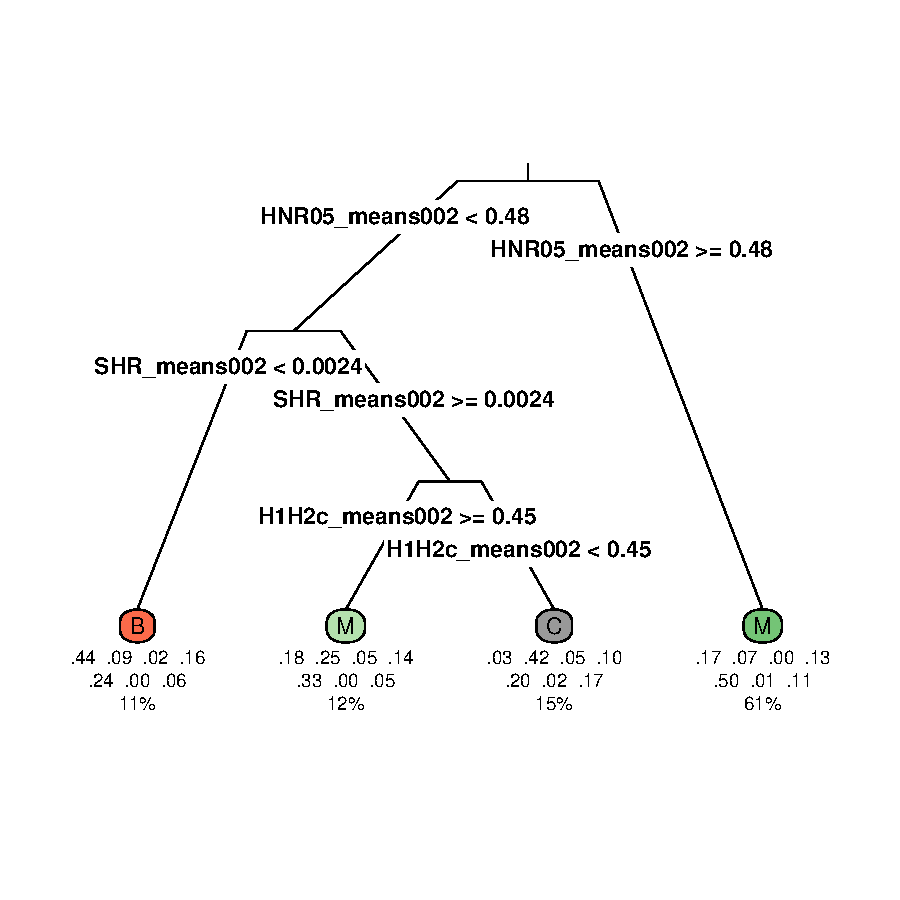
\includegraphics[width = 0.9\linewidth]{images/keating_tree.pdf}
    \caption{Classification tree of phonation categories from \citet{keatingCrosslanguageAcousticSpace2023}. Abbreviations used in this figure are: {HNR05_means002}: harmonics-to-noise ratio over the frequency range from 0 Hz to 500 Hz for the middle third of each vowel; {SHR_means002}: subharmonic-to-harmonic ratio for the middle third of each vowel; {H1H2c_means002}: H1* − H2* for the middle third of each vowel; B: breathy, M: modal, and C: creaky phonation categories.}
    \label{fig:keating_tree}
\end{figure}

Decision trees like the one in Figure~\ref{fig:keating_tree}, show the binary splits that are made in the space and what predictor, and the value of that predictor, makes that split. In the case of \citeauthor{keatingCrosslanguageAcousticSpace2023}'s (\citeyear{keatingCrosslanguageAcousticSpace2023}) tree, the first split is made on the harmonics-to-noise ratio over the frequency range from 0 Hz to 500 Hz for the middle third of each vowel. This split is made at the z-score of 0.48. If the value of the predictor is greater or equal to 0.48, the dominate voice quality of that region is modal. If, however, that HNR < 500 Hz value is less than 0.48, the region needs to be further split. 

The next split in the region is made on the subharmonic-to-harmonic ratio for the middle third of each vowel. If the value of this predictor is less than 0.0024, the voice quality is classified as breathy. If the value is greater than or equal to 0.0024, the region needs to be split further.

The final split in the region is made on the H1* - H2* for the middle third of each vowel. If the value of this predictor is less than 0.45, the voice quality is classified as creaky. If the value is greater than or equal to 0.45, the voice quality is classified as modal.

This tree shows that using only three acoustic measure, one can classify the voice quality of the data. This is a powerful tool for understanding the importance of the different acoustic measures in the acoustic space. 

%--------------------------
\section{Bagging Trees} \label{sec:bagging_bagging}
%--------------------------

Simple decision trees, however, suffer from two main disadvantages. The first is that decision trees can suffer from high variance. In other words, the tree can be very sensitive to small changes in the data that it was trained on. The second disadvantage is that decision trees do not have the same predictive accuracy as other regression or classification models (see \cite{hastieElementsStatisticalLearning2009} for discussion).

One way to overcome these disadvantages, is to make use of a technique called bootstrap aggregating, or bagging \citep{breimanBaggingPredictors1996}. This means that instead of growing a single tree on the data like in simple decision trees, we grow many trees on random samples of the data until we reach a given number of trees. Once these trees are grown, we then average across the trees to get a more stable prediction of how the regions are split and what predictors are most important in making those splits. This averaging across the trees help to explain the variance in the data and improve the predictive accuracy of the model. However, this comes at the cost of interpretability. 

In decision trees, we usually represent the splits in the data as a tree. When we using bagging, because of the large numbers of trees that are grown, it is impossible to represent the results in this way. Instead of using a tree, we use variable importance measures to understand which predictors are most important in making the splits in the data. There are two measures that are commonly used to understand variable importance in bagging trees: the residual sum of squares (RSS) for regression trees and the Gini index for classification. In regression trees, the amount that the RSS is decreased due to the splits over a given predictor is recorded and averaged across all the trees. In classification trees, the total amount that the Gini index is decreased for each predictor and averaged across all the trees. The higher the value of the RSS or Gini index, the more important that predictor is in making the splits in the data. These are then graphed to show the importance of each predictor in the data with the most important predictors at the top of the graph.

In many instances of bagging trees, the exact number of trees needed to be grown is not known \textit{a priori}. Instead, the number of trees is determined by the user and is usually determined by the number of trees that are needed to stabilize the prediction. This is done by comparing multiple models that where built with different numbers of trees and determining which number of trees produces the most stable prediction. This is done by comparing the predictions of the different models and calculating the variance of the predictions across the different models. The model that produces the most stable prediction is the one that is chosen.

In this chapter, I will use bagging trees to understand the importance of the different acoustic measures in making the splits in the acoustic space of SLZ. This will help to understand which measures are most important in separating the different voice qualities from one another.

%--------------------------
\section{Bagging Trees in SLZ} \label{sec:bagging_slz}
%--------------------------

Using the same data as in Chapter~\ref{ch:acousticlandscape}, I will use bagging trees to understand the importance of the different acoustic measures in making the splits in the acoustic space of SLZ. In order to determine the number of trees that are needed to stabilize the prediction, I compared models with different numbers of trees. The results of this comparison are shown in Figure~\ref{fig:bagging_tree}.

\begin{figure}[!ht]
    \centering
    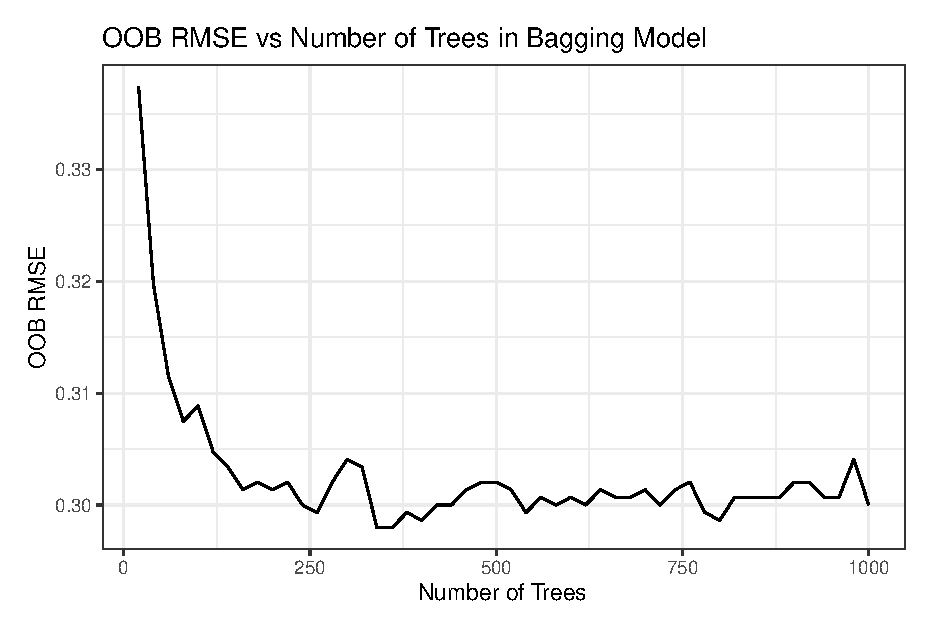
\includegraphics[width = 0.9\linewidth]{images/bagging_numbers.eps}
    \caption{Plot showing the out-of-bag error as a function of the number of trees ran in the bagging models.}
    \label{fig:bagging_tree}
\end{figure}

From Figure~\ref{fig:bagging_tree}, it is clear that the out-of-bag error stabilizes at approximately 400 trees. This means that the number of trees that are required for the the bagging model to be the most stable is also 400 trees. In order to further insure the stability of the model, I also ran a 10-fold cross-validation on the bagging model with 400 trees. The results of this model are shown in Figure~\ref{fig:bagging_importance}.

\begin{figure}[!ht]
    \centering
    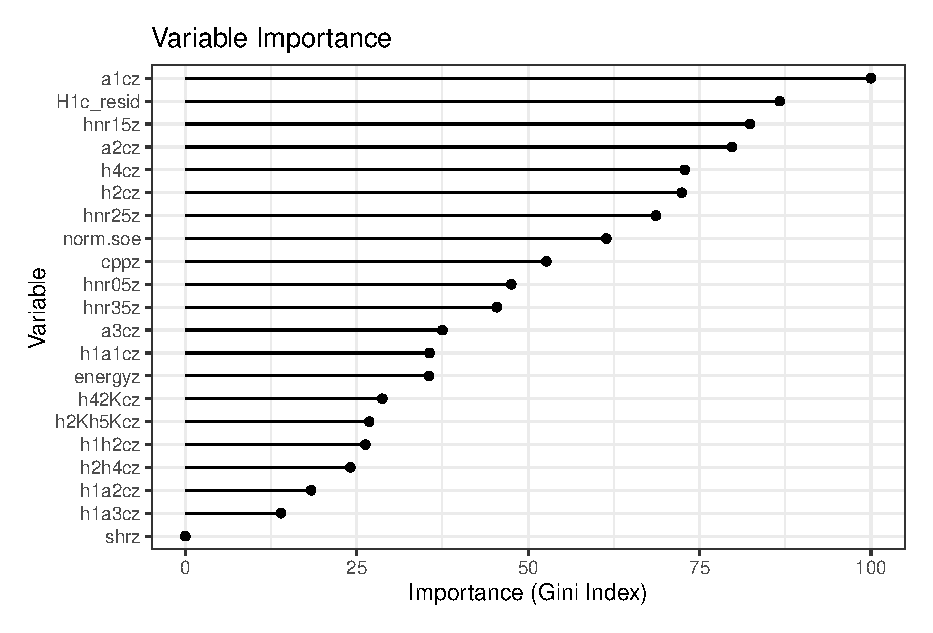
\includegraphics[width = 0.9\linewidth]{images/vip_bagging.eps}
    \caption{Variable importance plot showing the importance of the different acoustic measures in the bagging model based on the total amount that the Gini index is decreased by splits over a given predictor, averaged over all 400 trees.}
    \label{fig:bagging_importance}
\end{figure}

From Figure~\ref{fig:bagging_importance}, the variables with the largest mean decrease in Gini index are A1* (the amplitude of the harmonic closest to the first formant), residual H1*, and the harmonics-to-noise ratio over the frequency range from 0 Hz to 1500 Hz (HNR 1500 Hz). This means that these three variables are the most important in making the splits in the acoustic space of SLZ. This is consistent with the results of the MDS analysis in Chapter~\ref{ch:acousticlandscape}, where these three variables were some of the variables that contributed the most to the different dimensions of the acoustic space. 

%--------------------------
\section{Discussion} \label{sec:bagging_discussion}
%--------------------------

It is interesting to not that in both the MDS analysis and the bagging trees, the same three variables are found to play a role in the acoustic space of SLZ. These two analyses complement each other and help us to better understand what measures to focus are attention on. From Chapter~\ref{ch:acousticlandscape}, we saw that the acoustic measure A1* was heavily weighted for both dimensions 1 and 2. It is not surprising then that this measure would rank so high in the variable importance.

The other two measures that the bagging analysis found to be of most importance are the measures residual H1* and HNR 1500 Hz. These two measures were also important for the analysis in Chapter~\ref{ch:acousticlandscape}. However, they were only heavily weighted for dimension 3. 

The rest of this section will discuss each of the measures that were found to be important in the bagging analysis and how they relate to the different voice qualities in SLZ and other linguistic phenomena. 

%--------------------------
\subsection{Importance of A1*} \label{sec:bagging_a1}
%--------------------------

The measure that was found to be the most important for classifying SLZ's phonation contrasts was A1*. This measure captures the amplitude of the harmonic closest to the first formant. This measure is typically not found in voice quality research except as a way to normalize the amplitude of the first harmonic (i.e., H1*). This goes back to \citet{fischer-jorgensenPhoneticAnalysisBreathy1968} who used this as one of the ways to correct for the high pass filtering, in addition to the widely used H1*$-$H2* measure. However, A1* as a standalone measure is not typically used in voice quality research. Therefore what we are to make of this measure's importance in SLZ is not clear as is its behavior in regards to the different phonations. 

When we look at how A1* is distributed across the different voice qualities in SLZ, as seen as Figure~\ref{fig:a1}, we see that modal vowels are found at the top of the chart with the other phonation contrasts located lower on the chart. The phonation that is found at the bottom of the chart is breathy voice. 
\begin{figure}[!ht]
    \centering
    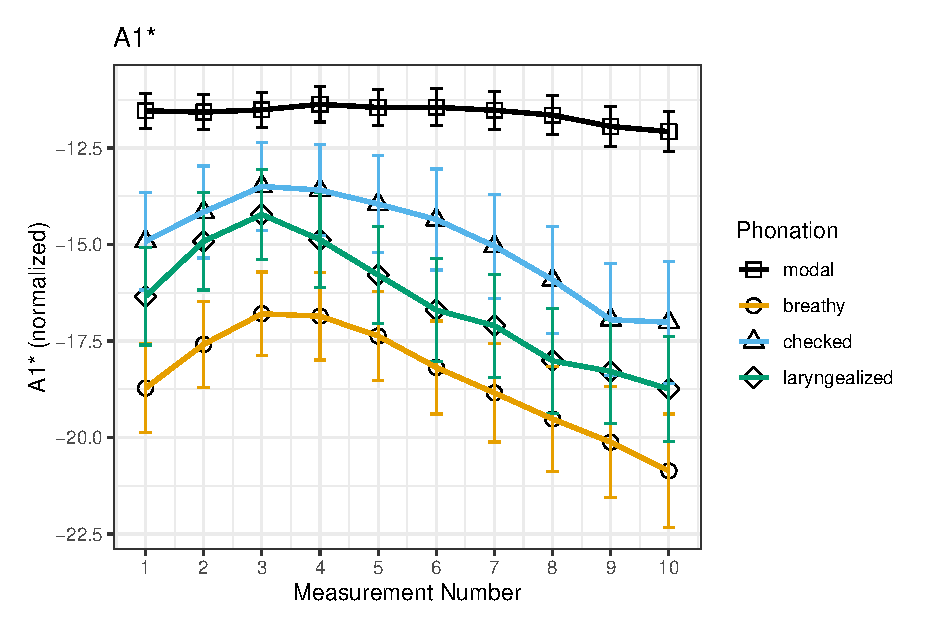
\includegraphics[width = 0.9\linewidth]{images/slz_a1c.eps}
    \caption{Plot showing the distribution of A1* across the different voice qualities in SLZ.}
    \label{fig:a1}
\end{figure}

This pattern of behavior, especially for breathy versus modal, is very similar to what is found in other languages and descriptions of the behavior of the first formant in breathy voice contexts. For example differences in the first formant are typically used to distinguish register differences in Southeast Asian languages \citep{brunelleRegisterEasternCham2005,brunelleDialectExperiencePerceptual2012,brunelleTonePhonationSoutheast2016}.

As described in \citet{brunelleTonePhonationSoutheast2016}, many of the languages of Southeast Asia have what is called register. The linguistic term register is defined as ``the redundant use of pitch, voice quality, vowel quality, and durational differences to distinguish (typically two) contrastive categories'' \citep[193]{brunelleTonePhonationSoutheast2016}, and was first used by \citet{hendersonMainFeaturesCambodian1952} to describe the categorical contrasts found in Khmer. The characteristics that define the higher and lower registers are found in Table~\ref{tab:register_correlates}.

\begin{table}[!ht]
    \centering
    \caption{Possible phonetic correlates of register. From \citet{brunelleTonePhonationSoutheast2016}.}
    \label{tab:register_correlates}
    \begin{tabular}{ll}
        \lsptoprule
        \textbf{Higher Register} & \textbf{Lower Register} \\
        \hline
        Higher pitch & Lower pitch \\
        Tense/Modal voice & Lax/Breathy voice \\
        Monophthongs/shorter vowels & Diphthongs/longer vowels \\
        Raised F1/lower vowels/[+ATR] & Lowered F1/higher vowels/[-ATR] \\
        Plain stops/shorter VOT & Aspirated stops/longer VOT \\
        \lspbottomrule
    \end{tabular}
\end{table}

From this table, the lower register is what interests us here. The lower register is associated with breathy voice and a lowered first formant. This is very similar to what we see in Figure~\ref{fig:a1} where breathy voice is associated with a lower A1* than modal voice. It is not entirely clear if the amplitude of the first formant also behaves in this same way in these languages as the the lowering of the first formant's frequency. 

There is evidence that breathy voice frequently has a lower first formant than modal voice in paralinguistic settings for English \citep{lottoEffectVoiceQuality1997}.  However, these studies do not discuss the amplitude of the first formant but rather the frequency of the first formant.

Another comparison can be found in nasality research, where this measure is discussed quite extensively either alone or in association with the nasal pole (e.g., \cite{chenAcousticCorrelatesEnglish1997,delvauxPerceptionContrasteNasalite2009,macmillanIntegralityNasalizationF11999,pruthiAcousticParametersAutomatic2004,,schwartzAcousticsNormalNasal1968,stevensAcousticPhonetics2000,stylerAcousticalPerceptualFeatures2015,stylerAcousticalFeaturesVowel2017}). These studies discuss how in nasalized contexts the amplitude of the first formant is typically found to be lower than in oral ones, again similar to what we see in Figure~\ref{fig:a1}.

There is a large body of research that discusses that nasality is closely associated with breathy voice or the glottal consonants, in a phenomenon called \textit{rhinoglottophilia} \citep{matisoffRhinoglottophiliaMysteriousConnection1975,ohalaPhoneticExplanationsNasal1975,ohalaPhoneticsNasalPhonology1993,bennettMayanPhonology2016}. In \citet{blevinsEvolutionPonapeicNasal1993,matisoffRhinoglottophiliaMysteriousConnection1975}, this association is attributed to the acoustic and perceptual similarities between nasalization and breathy voice. In one study, \citet{garellekBreathyVoiceNasality2016} showed that in nasalization in three different Yi languages were associated with breathy voice. Leading the authors to suggest that breathy voice during nasalization can arise from misperception or as a type of phonetic enhancement. 

In regards to what is going on in SLZ, it is not clear if the lowering of A1* for breathy voice can be attributed to the same observations as discussed above. I suggest that there are three different possibilities to explain what is going on in SLZ. Because SLZ does not have phonemic nasaliZation, it is possible that speakers of SLZ are using nasalization as a way to phonetically enhance the the contrast of breathy voice. Essentially, the reverse of what was reported by \citet{garellekBreathyVoiceNasality2016}. This possibility could be tested acoustically by performing an experiment to detect nasal airflow during breathy vowels. The second possibility is that the same measures that work for detecting nasality can also be used to detect breathy voice. This second possibility could be easily tested by examining whether A1* and the other measures for nasality work in other breathy voice contexts cross-linguistically. The third possibility is that the lowering of A1* is a result of sub-glottal resonances which is much harder to test than the other two possibilities. 

%--------------------------
\subsection{Importance of Residual H1*} \label{sec:bagging_residual}
%--------------------------
\begin{figure}[!ht]
    \centering
    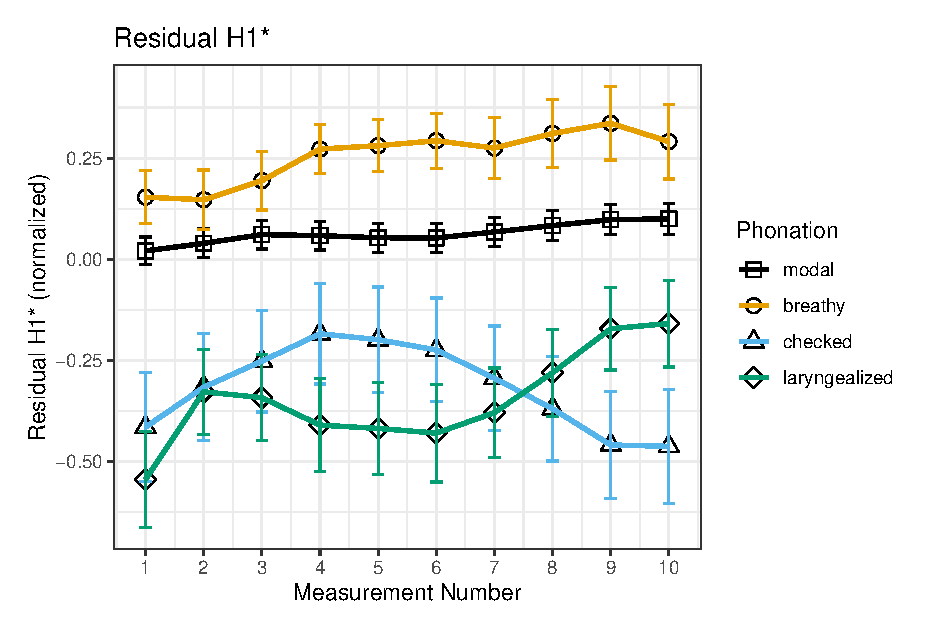
\includegraphics[width = 0.9\linewidth]{images/slz_residual_h1c.eps}
    \caption{Plot showing the distribution of residual H1* across the different voice qualities in SLZ.}
    \label{fig:residualH1}
\end{figure}

%--------------------------
\subsection{Importance of HNR \textless 1500 Hz} \label{sec:bagging_hnr}
%--------------------------

\begin{figure}[!ht]
    \centering
    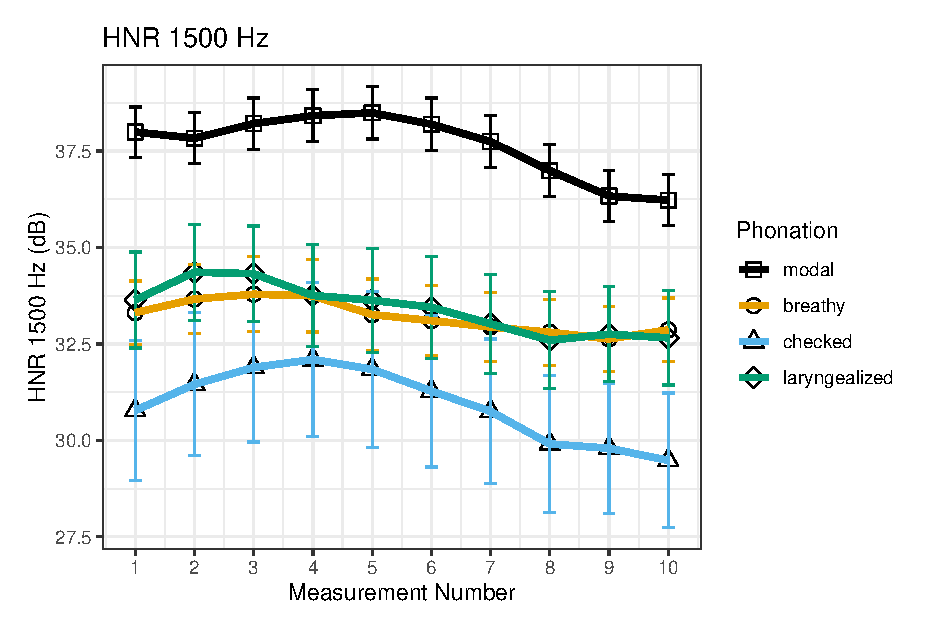
\includegraphics[width = 0.9\linewidth]{images/slz_hnr15.eps}
    \caption{Plot showing the distribution of HNR 1500 Hz across the different voice qualities in SLZ.}
    \label{fig:hnr1500}
\end{figure}

%--------------------------
\section{Conclusion} \label{sec:bagging_conclusion}
%--------------------------


